\section{Resultatbehandling}
    
    \subsection{Syntese 1}
    \subsubsection{Smeltepunktsanalyse}
    \begin{table}[H]\centering
        \begin{tabular}{ccc}
                \toprule
                Prøve # & Smeltepunkt $\left[\si{\degree C}\right]$ & Afvigelse $\left[\%\right]$ \\
                \midrule
                1 & 116 & -1 \\
                2 & 115 & -2 \\
                3 & 117 & 0 \\
                \midrule
                Gennemsnit & 116 & -1 \\
                \bottomrule
            \end{tabular}
        \caption{Smeltepunktsanalyse af produket dannet ved syntese 1.}
    \end{table}

    \subsubsection{TLC--analyse}
    
    \begin{table}[H]\centering
        \resizebox{\textwidth}{!}{
        \begin{tabular}{ccccccc}
            \toprule
            Plade # & Løbelængde $\left[\si{cm}\right]$ & Kommercielt $\left[\si{cm}\right]$ & Eget $\left[\si{cm}\right]$ & rf kommercielt & rf eget & Afvigelse $\left[\%\right]$\\
            \midrule
            1 & 5.4 & 1.1 & 1.3 & 0.20 & 0.24 & 18 \\
            2 & 4.5 & 1.0 & 0.9 & 0.22 & 0.20 & -10 \\
            3 & 4.8 & 1.1 & 1.0 & 0.23 & 0.21 & -9 \\
            \midrule
              & & & Gennemsnit & 0.22 & 0.22 & 0 \\
            \bottomrule
        \end{tabular}
        }
        \caption{TLC--analyse af propylparaben dannet ved syntese 3.}
    \end{table}

    \subsection{Syntese 2}
    \subsubsection{Smeltepunktsanalyse}
    \begin{table}[H]\centering
        \begin{tabular}{ccc}
                \toprule
                Prøve # & Smeltepunkt $\left[\si{\degree C}\right]$ & Afvigelse $\left[\%\right]$ \\
                \midrule
                1 & 95 & -2 \\
                2 & 96 & -1 \\
                3 & 96 & -1 \\
                \midrule
                Gennemsnit & 95.7 & -1 \\
                \bottomrule
            \end{tabular}
        \caption{Smeltepunktsanalyse af produket dannet ved syntese 2.}
    \end{table}

    \subsubsection{TLC--analyse}
    
    \begin{table}[H]\centering
        \resizebox{\textwidth}{!}{
        \begin{tabular}{ccccccc}
            \toprule
            Plade # & Løbelængde $\left[\si{cm}\right]$ & Kommercielt $\left[\si{cm}\right]$ & Eget $\left[\si{cm}\right]$ & rf kommercielt & rf eget & Afvigelse $\left[\%\right]$\\
            \midrule
            1 & 4.9 & 3.1 & 3.4 & 0.63 & 0.69 & 10 \\
            2 & 4.8 & 3.2 & 3.1 & 0.67 & 0.65 & -3 \\
            3 & 4.9 & 2.9 & 2.9 & 0.59 & 0.59 & 0 \\
            \midrule
              & & & Gennemsnit & 0.63 & 0.64 & 2 \\
            \bottomrule
        \end{tabular}
        }
        \caption{TLC--analyse af propylparaben dannet ved syntese 3.}
    \end{table}

    \subsection{Syntese 3}
    \subsubsection{Smeltepunktsanalyse}

    \begin{table}[H]\centering
        \begin{tabular}{ccc}
                \toprule
                Prøve # & Smeltepunkt $\left[\si{\degree C}\right]$ & Afvigelse $\left[\%\right]$ \\
                \midrule
                1 & 116 & -1 \\
                2 & 116 & -1 \\
                3 & 117 & 0 \\
                \midrule
                Gennemsnit & 116.3 & -1 \\
                \bottomrule
            \end{tabular}
        \caption{Smeltepunktsanalyse af ethylparaben dannet ved syntese 3.}
    \end{table}
    
    \begin{table}[H]\centering
        \begin{tabular}{ccc}
            \toprule
            Prøve # & Smeltepunkt $\left[\si{\degree C}\right]$ & Afvigelse $\left[\%\right]$ \\
            \midrule
            1 & 96 & -2 \\
            2 & 93 & -4 \\
            3 & 94 & -3 \\
            \midrule
            Gennemsnit & 94.3 & -3 \\
            \bottomrule
        \end{tabular}
        \caption{Smeltepunktsanalyse af propylparaben dannet ved syntese 3.}
    \end{table}

    \subsubsection{TLC--analyse}
    
    \begin{table}[H]\centering
        \resizebox{\textwidth}{!}{
        \begin{tabular}{ccccccc}
            \toprule
            Plade # & Løbelængde $\left[\si{cm}\right]$ & Kommercielt $\left[\si{cm}\right]$ & Eget $\left[\si{cm}\right]$ & rf kommercielt & rf eget & Afvigelse $\left[\%\right]$\\
            \midrule
            1 & 5.0 & 2.5 & 2.5 & 0.50 & 0.50 & 0 \\
            2 & 4.7 & 2.3 & 2.3 & 0.49 & 0.49 & 0 \\
            3 & 4.9 & 2.4 & 2.4 & 0.49 & 0.49 & 0 \\
            \midrule
              & & & Gennemsnit & 0.49 & 0.49 & 0 \\
            \bottomrule
        \end{tabular}
        }
        \caption{TLC--analyse af ethylparaben dannet ved syntese 3.}
    \end{table}
    
    \begin{table}[H]\centering
        \resizebox{\textwidth}{!}{
        \begin{tabular}{ccccccc}
            \toprule
            Plade # & Løbelængde $\left[\si{cm}\right]$ & Kommercielt $\left[\si{cm}\right]$ & Eget $\left[\si{cm}\right]$ & rf kommercielt & rf eget & Afvigelse $\left[\%\right]$\\
            \midrule
            1 & 4.9 & 2.4 & 2.2 & 0.49 & 0.45 & -8 \\
            2 & 4.7 & 2.1 & 2.0 & 0.45 & 0.43 & -5 \\
            3 & 4.9 & 2.2 & 2.2 & 0.45 & 0.45 & 5 \\
            \midrule
              & & & Gennemsnit & 0.46 & 0.44 & -3 \\
            \bottomrule
        \end{tabular}
        }
        \caption{TLC--analyse af propylparaben dannet ved syntese 3.}
    \end{table}

    \subsection{H--NMR--spektroskopi}
    Vi undersøger først spektret for ethylparaben og vurderer om det er sandsynligt at det dannede H NMR-spektrum passer til det vi ville forvente. Til dette formål kigger vi på de individuelle peaks da antallet af spidser kan give os en ide om hvilke atomer de korresponderer til.
    \begin{figure}[H] \centering
        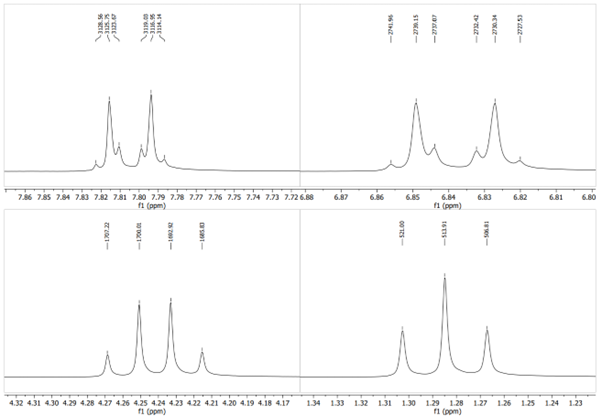
\includegraphics[width=\textwidth]{billeder/ethylpeaks}
        \caption{Peaks for H--NMR analyse af ethylparaben.}
    \end{figure} 
    Peaket omkring $\delta=1.28\si{ppm}$ forventes at være tilsvarende methylgruppen på forgreningen der udgår fra benzenringen, eftersom vi observerer 3 peaks, må atomet hydrogenerne er bundet til have 2 naboprotoner, hvilket kun opfyldes af methylengruppen. Ved $\delta=4.25\si{ppm}$ ses 4 peaks, altså må det være methylengruppen idet den har 3 naboprotoner fra methylgruppen. 
    
    Omkring $\delta=6.84\si{ppm}$ forventer vi hydrogenerne bundet til carbonatomerne i meta-positionerne i benzenringen, idet de vil have et lavere kemisk skift end dem i ortho-positionen grundet den øgede elektronegativitet fra oxygenatomet der er til stede i phenolgruppen. 
    
    I selve spektret ses også en singlet ved $\delta=10.25\si{ppm}$, dette kemiske skift er højere end hvad vi normalt villet forvente for en phenolgruppe (der normalt villet befinde sig omkring det aromatiske område, ligesom ortho- og meta-carbonatomerne). Dette kan begrundes i det benyttede opløsningsmiddel, DMSO-d6, da det har mulighed for at danne hydrogenbindinger med phenolgruppen \parencite{Raym2007}
    \begin{figure}[H]\centering
        \resizebox{\textwidth}{!}{
        \schemestart
        \chemfig{HO-*6(=-=(-COOR)-=-)}
        \+
        \chemfig[-32pt]{S(-[7]CD3)(-[5]CD3)(=[2]O)}
        \arrow(.mid east--.mid west){->}
        \chemfig{O(=[5]S(-[3]CD3)(-[6]CD3))-[2,,,,thick,dotted,red]H(-[1]O-*6(=-=(-COOR)-=-))}
        \schemestop
        }
        \caption{Dannelse af hydrogenbinding mellem DMSO-d6 og vilkårlig paraben.}
    \end{figure}
    Dette medfører at deres elektronegativitet ``mødes i midten'', hvorved den lokale elektrondensitet på hydrogenatomet (og derved beskyttelsen mod $B_0$) øges drastisk.
    \begin{figure}[H] \centering
        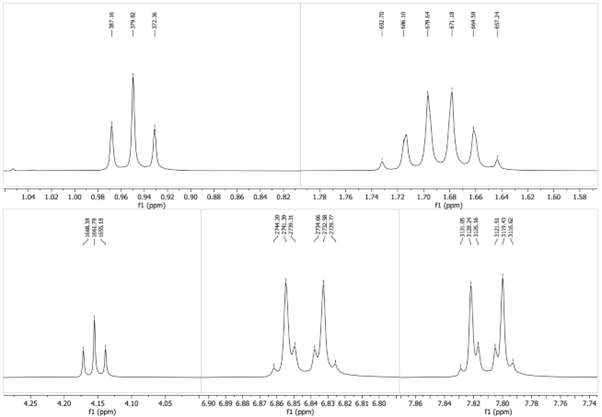
\includegraphics[width=\textwidth]{billeder/propylpeaks}
        \caption{Peaks for H--NMR analyse af propylparaben.}
    \end{figure} 
    TODO: kommenter på spektrum

    \subsection{IR--spektroskopi}


    \subsection{Hæmningsforsøg}
    

